\documentclass[man,floatsintext]{apa6} % Options: jou (journal), man (manuscript), doc (document) can use man,floatintext to get charts in right place but 25 pages
\usepackage[american]{babel} % Set language
\usepackage{csquotes}        % Required for APA citations
\usepackage{subcaption}      % For subfigures
\usepackage{apacite}         % For APA-style references
\usepackage{graphicx}        % For including figures
%\setlength{\belowcaptionskip}{10pt} % Adjust space below captions
%\setlength{\floatsep}{10pt} % Adjust space between floats
\usepackage{amsmath}         % For mathematical equations
\usepackage{float}
\usepackage{array}
\usepackage{caption}
\captionsetup[figure]{justification=centering, singlelinecheck=false}
\captionsetup[table]{justification=centering, singlelinecheck=false, labelsep=space}
%\usepackage{breakurl}
\usepackage[hyphens]{url} % Allows hyphenation in URLs


\title{Predicting Student Outcomes on Standardized Testing using Machine Learning}
\shorttitle{}
\author{Stacy Roberts}
\affiliation{The University of Texas at Austin \\ December 2024}

\abstract{
Finding a solution to the problem of student success has long been a goal and a frustration in education. Helping teachers, administrators, and support staff more easily identify which students will benefit from additional intervention to achieve successful outcomes helps focus limited resources. Being able to focus on the right students most in need of closer monitoring or more preparation assistance produces better utilization of public school's limited resources such that they may see the highest return on investment. Accounting for factors outside of school control is also necessary to understanding how best to serve the student population of a given school. Markers of success in this project will center around standardized testing scores in Math, Reading, and Writing. Providing another tool for public schools to more quickly and easily narrow focus on the students most in need of additional intervention to gain and retain the skills necessary to pass standardized testing is integral to good use of the limited resources available for these students.}

\begin{document}
\maketitle

\section{Introduction}

Predicting student outcomes is a necessary function of the public school system, which is tasked with maximizing the success of their entire student population. All schools are invested in the percentage of their students who graduate on time and go on to higher education or employment, as it is reflective of the success of the school itself. However, gaining access to student data is easier with public schools given the government mandates of public reporting they are required to follow, most recently detailed in the Every Child Succeeds Act \cite{ecsa}. This paper will focus on public schools as they are required to service anyone within the community, yielding a true representation of the population in a given area.

There are many ideas of what types of students require additional assistance to be successful in school. Focus is generally placed on socioeconomic status (SES), race, gender, and parental education level as discussed in \cite{Bradley2022SESgap}.  Time and again, higher socioeconomic areas have higher student achievement outcomes. This is true for both the high and low socioeconomic groups when the average status is elevated for the area.  Higher Socioeconomic Groups have many advantages, from stable homes and plentiful food to higher quality and more stable teaching and administrative staff at the schools which service them, per \cite{HSEffectsLongTerm}. This paper is not intending to investigate all possible differentials, but does note that it is difficult to separate all the co-variant factors which contribute to the success of a student population. Is it more important to have a stable, effective teaching staff or to provide a support system where all students have stability and enough food to eat? Ideal data sets for investigating this theory would involve students of equally matched SES with large differentials in staff quality, as well as students with the same teachers but large differential in SES to attempt to isolate how important SES is for student success. Families are generally averse to subjecting their children to be educational theory test subjects. However, there is value in surveying students and families to understand their experiences and attitudes regarding seeming tangential behaviors. Behaviors such as smoking, alcohol access, and coping strategies would be beneficial to include in an input dataset. These types of behaviors have been shown in \cite{tiertaryBehaviors} to also be influential in how students fair academically.

Yet there are some pockets of students who outperform expectations based on background discussed in \cite{YanGaiLowSEG}. These students often have strong support systems with an emphasis on educational importance and future educational attainment. They have a positive outlook and experience within academia, and likely a harmonious relationship with at least one of their teachers. One take away from this group of students is that imparting a positive experience and fostering a connection with even one staff member is important in convincing them of the importance of academic success on their future options. These soft skills are just as integral to a student's academic success as curriculum and prior academic performance.

Our project aims to utilize different Machine Learning models to identify students who are risk of failing standardized math, reading, and writing assessments based on available background information.  The intention is that this become one more tool available to schools for filtering their student populations to more easily identify which students would benefit from further intervention and thereby increase their success as measured by standardized testing.

\section{Research Background}
Efforts to improve student outcomes have had varying rates of success. There is no single path which guarantees that all students achieve high school graduation and beyond.  Instead, there is a continuous cycle of new research, new methods, and new options attempting to increase material retention, attendance, and ultimately, state testing scores. This cycle has been going on for as decades. As noted in \cite{AustraliaSES} and \cite{Malaysia}, this is an international problem as well. Schools all around the world are interested in mining information from their educational databases to improve their standing by increasing student performance and/or graduation metrics.  

Study after study has found that students who enter kindergarten behind their peers will struggle to make up the gap throughout their entire schooling, as shown in \cite{EdInequities}, \cite{sesbehind1}, \cite{sesbehind2}, and \cite{sesbehind3}. High quality and accessible pre-K, along with increasing availability of books at home have been shown to make significant improvements in preparing students for kindergarten, per \cite{earlyengageML}. However as discussed in \cite{cradleK}, there are precious few resources for families in the lower and middle socioeconomic spectrum to access these trajectory changing elements for their children. Providing more social safety nets such as paid parental leave, affordable child care, and more expanded and intensive services for families experiencing multiple adversities similar to every other developed nation would significantly improve the standing of children born into the more dire of situation as discussed in \cite{duncan2013long} and \cite{duncan2012importance}.

Socioeconomic status also affects access to Twentieth Century necessities like internet access and personal laptops. Given that nearly all school systems use online classrooms and school work, having access to a personal computer and internet at home is a requirement to be successful in school. However, personal computers come with a significant price tag, and internet, even with income-based discounts, is a monthly expense many families cannot afford, as discussed in \cite{sesinternet}. Opportunities such as a completely online program, which should level the field and allow people of disparate locations access to education, are also impossible to reach for those without computers or internet. Yet even in those programs, there is desire to understand the student population and identify who would be more successful at completing, per \cite{DistLearnML}.

Returning to the metrics we chose to focus on, school systems focus on elevating standardized testing scores as that is how they are ranked for public viewing per \cite{linnetal}. These rankings then influence who chooses to buy homes within the district, which in turn influences the socioeconomic level of the population and the educational attainment and retention of the teaching, support, and admin staff attracted to said schools per \cite{perry2010does}. The unfortunate side effect is that limited resources get reallocated to focus on preparation and support surrounding standardized testing, to the detriment of more holistic approaches in support of the entire student as discussed in \cite{cradle}. There are some alternative theories of educational success metrics making inroads into the Data Mining field. One such is Outcome-Based Education where the focus is on the student's knowledge and skills at the point of graduation as discussed in \cite{studentPerfOBE}. This is a newer focus and has different requirements of input data, but would be an interesting expansion opportunity. 

\section{Methods}
\subsection{Data Analysis}
The data selected for analysis contains 1000 anonymous student information. It includes background information on each student with regards to parental education, reduced/free lunch participation, whether they completed a test preparation course, gender, and test scores for math, reading, and writing assessments. There is enough information to make an educated guess as to the socioeconomic level of each student. Given the data provided, we decided whether the student was on reduced/free lunch plan could substituted as a proxy for actual demographic data indicating their SES. Students can only qualify for the reduced/free lunch plan if their guardians are below a specified income level. While this will not correctly classify all students, based on available information it is the best method to distinguish we have accessible. The following studies, \cite{maternaleducation} \cite{maternaleducation2} \cite{maternaleducation3}
, all include the mother's level of education as a major indicator of a student's SES, but this data set doesn't have that sort of granularity. As such we decided to take a significant look at the Parental Level of Education, although we were unable to separate which parent this references.

First we performed data analysis on the chosen dataset. Of interest was seeing if the data analysis showed any correlation between the parents' education level and the passing rates of their children. Each individualized standardized testing area was evaluated separately to see if there were different correlations for the different subjects, shown in Figure \ref{fig:FirstOne}. 

\begin{figure}[H]
    \centering
    \caption{Correlations of Parent Education to Student Scores}
    \begin{subfigure}[b]{0.28\textwidth}
    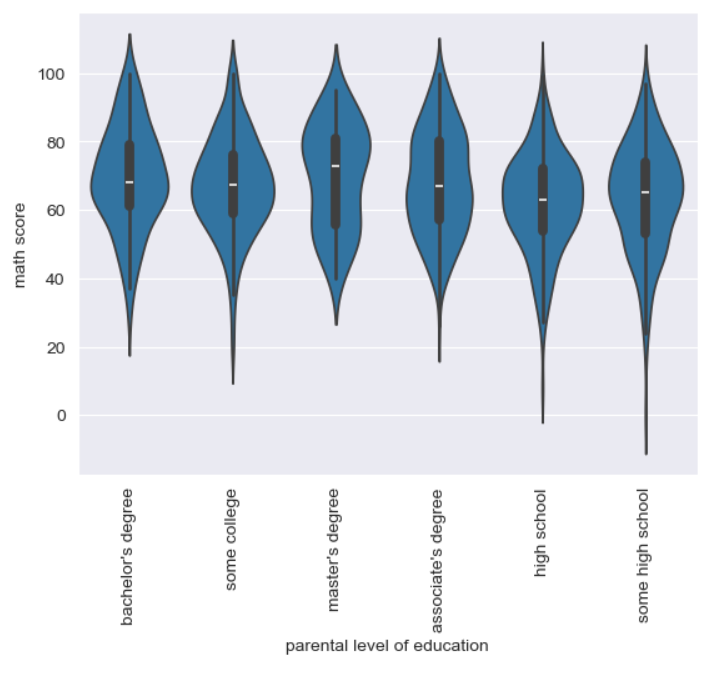
\includegraphics[width=\linewidth]{MathVsParent.png}
    \caption{Correlation of Math Scores}
    \label{fig:math1}
    \end{subfigure}
    \begin{subfigure}[b]{0.28\textwidth}
    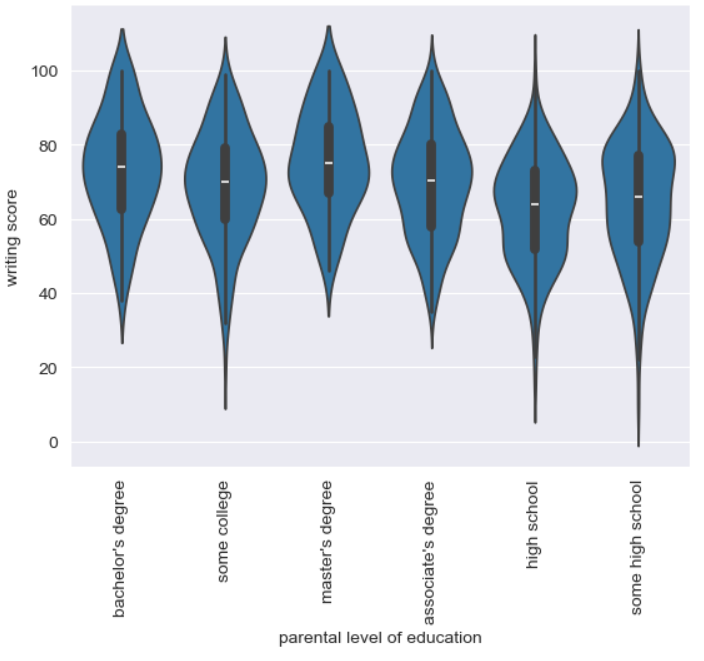
\includegraphics[width=\linewidth]{WritingVsParent.png}
    \caption{Correlation of Writing Scores}
    \label{fig:read1}
    \end{subfigure}
    \begin{subfigure}[b]{0.28\textwidth}
    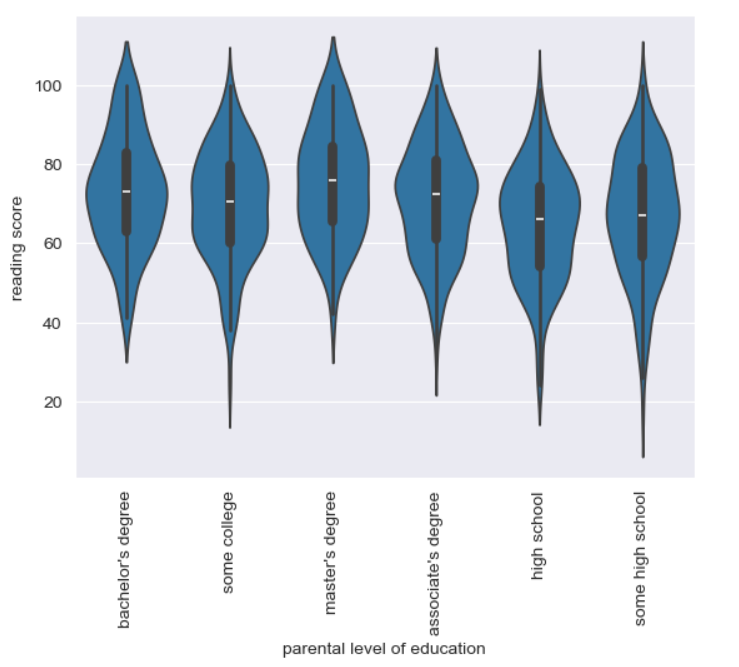
\includegraphics[width=\linewidth]{ReadingVsParent.png}
    \caption{Correlation of Reading Scores}
    \label{fig:write1}
    \end{subfigure}
    \label{fig:FirstOne}
\end{figure}

Figure \ref{fig:FirstOne} indicates a small difference in outcomes between the subject areas. While the overall average isn't significantly different when looking at the data in this manner, the variance becomes noticeable as the parental education level goes down. The students of families with the highest level of parental education also achieved the highest mean, while those whose parents only completed some high school had the widest variance in scores.

Focusing specifically on the Math Scores in Figure \ref{fig:math1}, while the students of all parental education levels were able to attain a similar top end score, the variability of the plot indicates a higher mean the more education the parents obtained.  Students of parents with a Master's degree had the highest mean math score, but the other education levels didn't show a significant difference in the mean.  The most noticeable difference between the categories is the lowest score rate. The lower the education level of the parents, the lower the lowest scores of the students.  Clearly there is some correlation, but not as strong of one in this particular dataset as might be expected based on the volume of literature around SES and student success.
Similar to the Math score graph, the Reading, Figure \ref{fig:read1}, and Writing, Figure \ref{fig:write1}, scores show variability relative to parental education level.  It is more noticeable that those whose parents only achieved at most a high school level of education had lower mean and bottom end scores in reading and writing. It would appear that within this dataset, the influence of parent's education is more noticeable in reading and writing ability than math.

It becomes more apparently how parental education level affects student performance when we compare strict pass rates, grouped by the parent's education level. These graphs are normalized for the differing numbers of parents in each group to provide a percentage passing rate for each group as seen in Figure \ref{fig:PassRatesParentEdLevel}.  Passing is considered achieving 70\% or higher on the standardized test.

\begin{figure}[H]
    \centering
    \caption{Correlations of Parent Education to Student Pass Rates}
    \begin{subfigure}[b]{0.28\textwidth}
    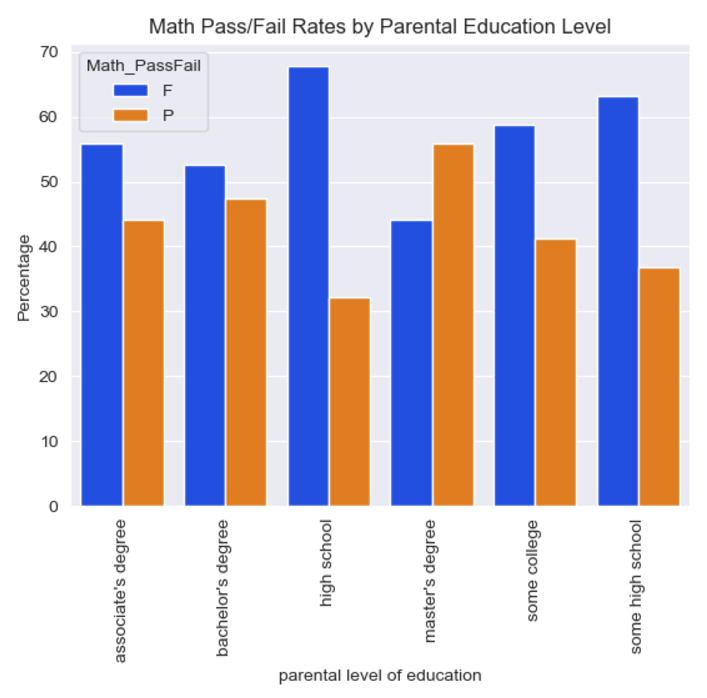
\includegraphics[width=\linewidth]{MathPFBarGraph.png}
    \caption{Passing Rates for Math Test}
    \label{fig:math}
    \end{subfigure}
    \begin{subfigure}[b]{0.28\textwidth}
    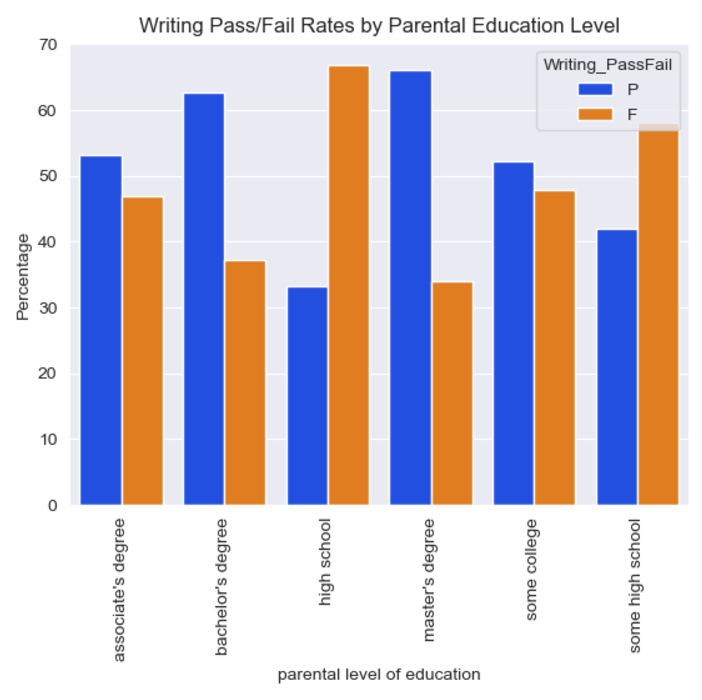
\includegraphics[width=\linewidth]{WritingPFBarGraph.png}
    \caption{Passing Rates for Writing Test}
    \label{fig:write}
    \end{subfigure}
    \begin{subfigure}[b]{0.28\textwidth}
    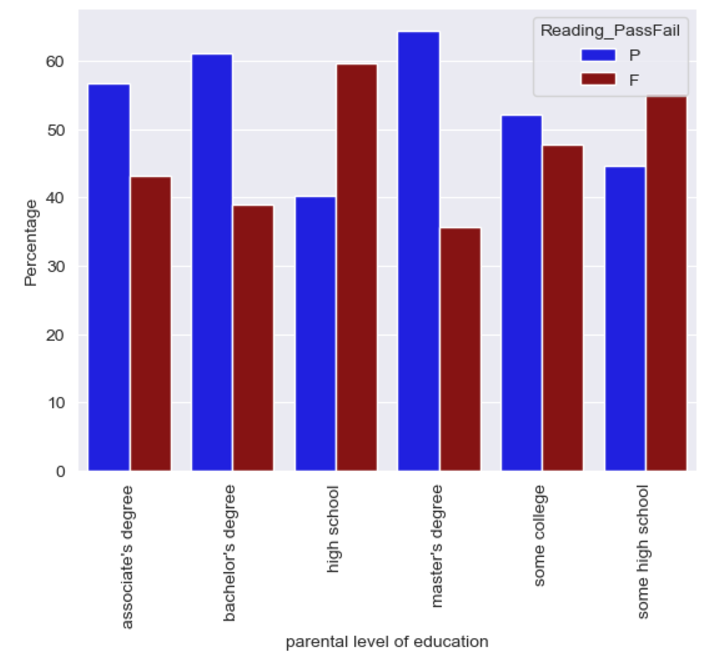
\includegraphics[width=\linewidth]{ReadingPFBarGraph.png}
    \caption{Passing Rates for Reading Test}
    \label{fig:read}
    \end{subfigure}
    \label{fig:PassRatesParentEdLevel}
\end{figure}

There were much lower passing rates on the Math assessment across the board per Figure \ref{fig:math}, with only students from families who obtained a Master's Degree achieving a greater than 50\% pass rate at all. In both the Writing and Reading assessments, Figure \ref{fig:write} and Figure \ref{fig:read}, students from families who completed some college or higher achieved a greater than 50\% pass rate with Master's Degree students having the highest success rate of all groups in both of these assessments. Based on this view the parental education level appears to have an out-sized impact on Reading and Writing test ability.

If we focus only on gender, another differential becomes apparent. Female students performed better than their Male counterparts overall as shown in Figure \ref{fig:FemaleMaleAvgScores}. Although Male students did performed better than Female students in the Math test, shown in Figure \ref{fig:FemaleMaleGraphsM}, Female students performed better on both the Writing and Reading tests as seen in Figure \ref{fig:FemaleMaleGraphsW} and Figure \ref{fig:FemaleMaleGraphsR}. This is regardless of parental education level.
\begin{figure}[H]
    \centering
    \caption{Average Standardized Scores by Gender}
    \begin{subfigure}[b]{0.4\textwidth}
        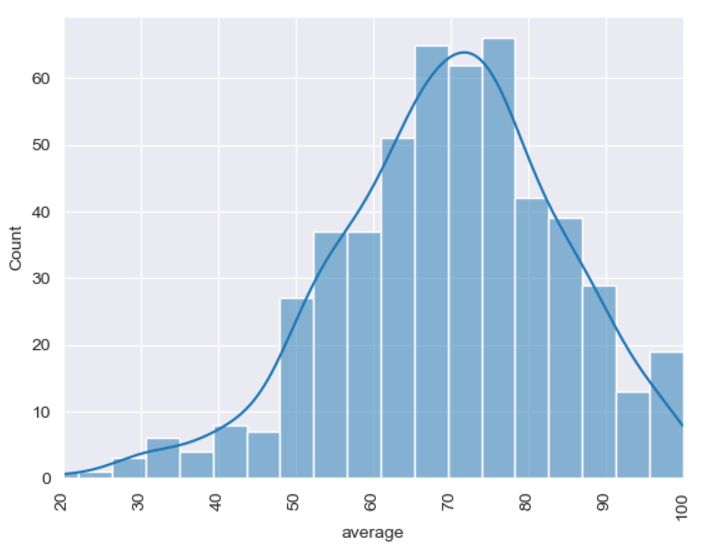
\includegraphics[width=\linewidth]{FemaleAverageScoreCurve.png}
        \caption{Female Students Avg Scores}
        \label{fig:FemaleAvg}
    \end{subfigure}
    \begin{subfigure}[b]{0.4\textwidth}
        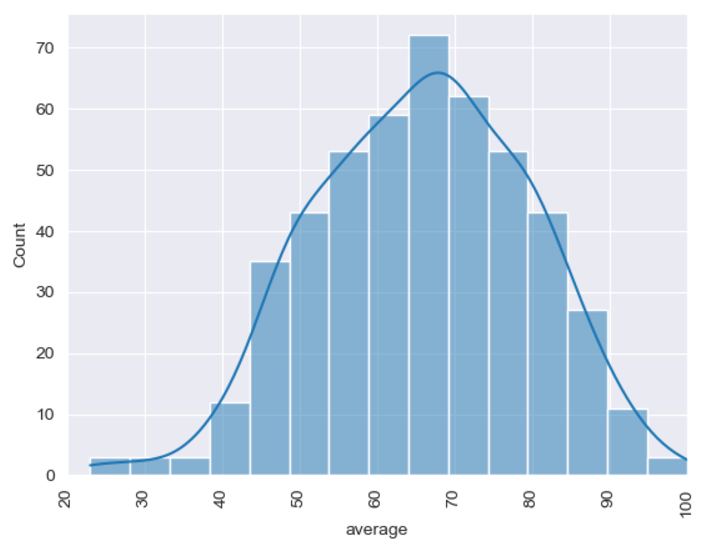
\includegraphics[width=\linewidth]{MaleAverageScoreCurve.png}
        \caption{Male Students Avg Scores}
        \label{fig:MaleAvg}
    \end{subfigure}
    \label{fig:FemaleMaleAvgScores}
\end{figure}
\begin{figure}[H]
    \centering
    \caption{Math Standardized Scores by Gender}
    \begin{subfigure}[b]{0.4\textwidth}
        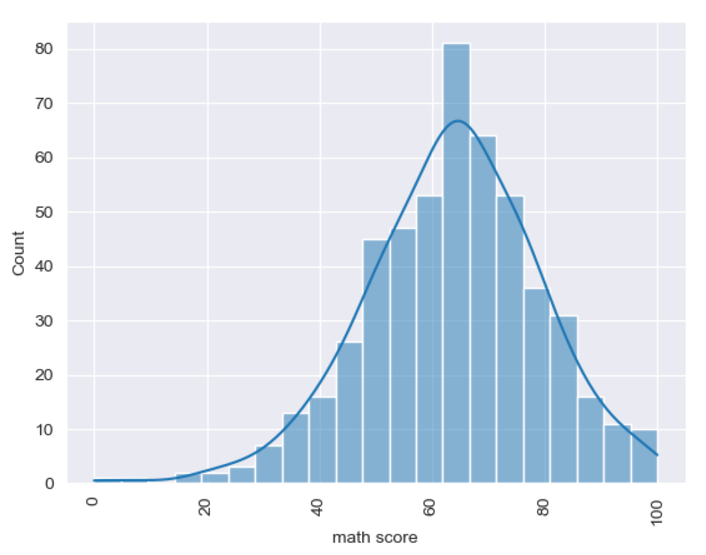
\includegraphics[width=\linewidth]{FemaleStudentsMathScoreCurve.png}
        \caption{Female Students Math Scores}
        \label{fig:FemaleMath}
    \end{subfigure}
    \begin{subfigure}[b]{0.4\textwidth}
        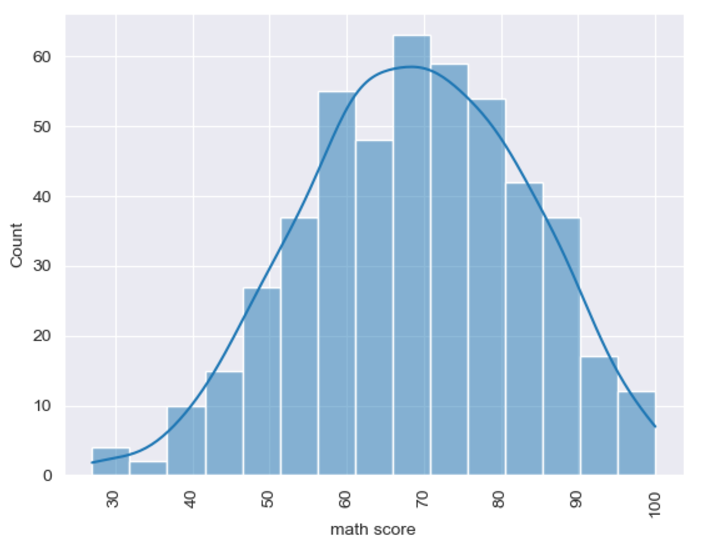
\includegraphics[width=\linewidth]{MaleStudentMathScoresCurve.png}
        \caption{Male Students Math Scores}
        \label{fig:MaleMath}
    \end{subfigure}
    \label{fig:FemaleMaleGraphsM}
\end{figure}
\begin{figure}[H]
    \centering
    \caption{Writing Standardized Scores by Gender}
    \begin{subfigure}[b]{0.4\textwidth}
        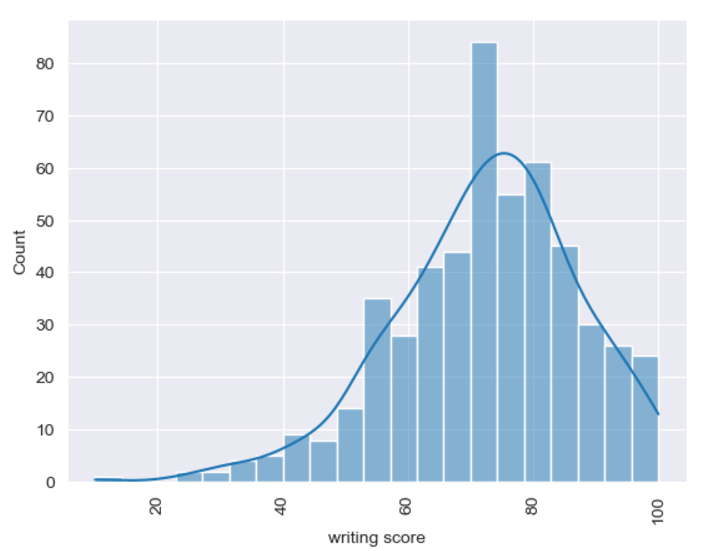
\includegraphics[width=\linewidth]{FemaleStudentsWritingScoreCurve.png}
        \caption{Female Students Writing Scores}
        \label{fig:FemaleWriting}
    \end{subfigure}
    \begin{subfigure}[b]{0.4\textwidth}
        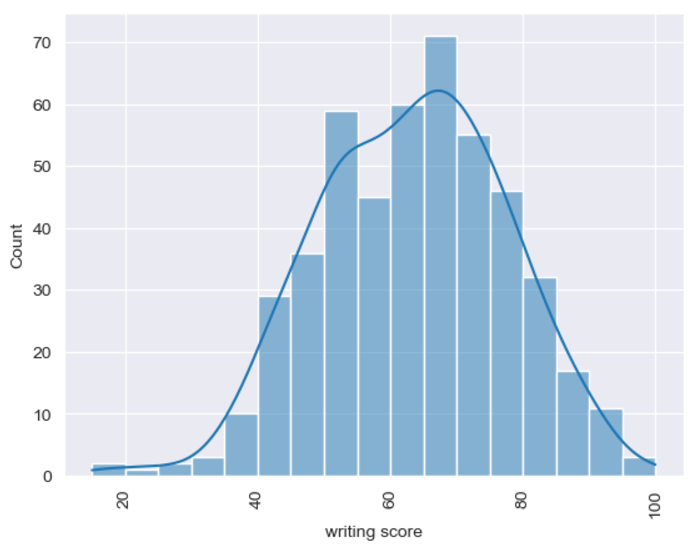
\includegraphics[width=\linewidth]{MaleStudentWritingScoreCurve.png}
        \caption{Male Students Writing Scores}
        \label{fig:MaleWriting}
    \end{subfigure}
    \label{fig:FemaleMaleGraphsW}
\end{figure}
\begin{figure}[H]
    \centering
    \caption{Reading Standardized Scores by Gender}
    \begin{subfigure}[b]{0.4\textwidth}
        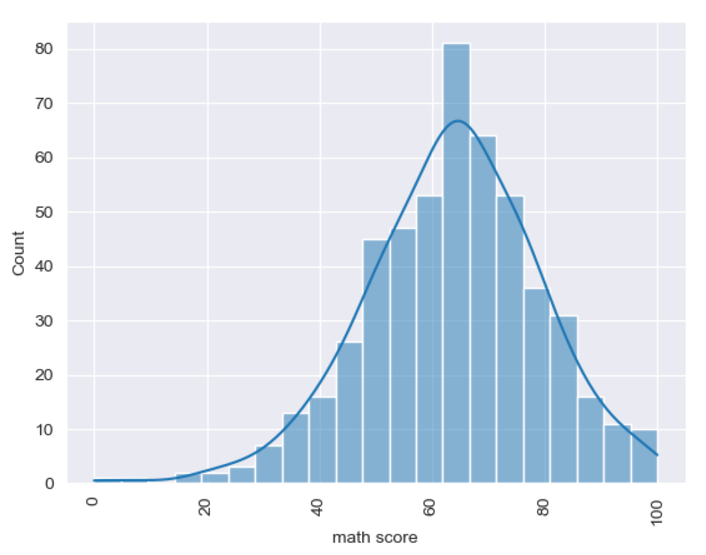
\includegraphics[width=\linewidth]{FemaleStudentsMathScoreCurve.png}
        \caption{Female Students Reading Scores}
        \label{fig:FemaleRead}
    \end{subfigure}
    \begin{subfigure}[b]{0.4\textwidth}
        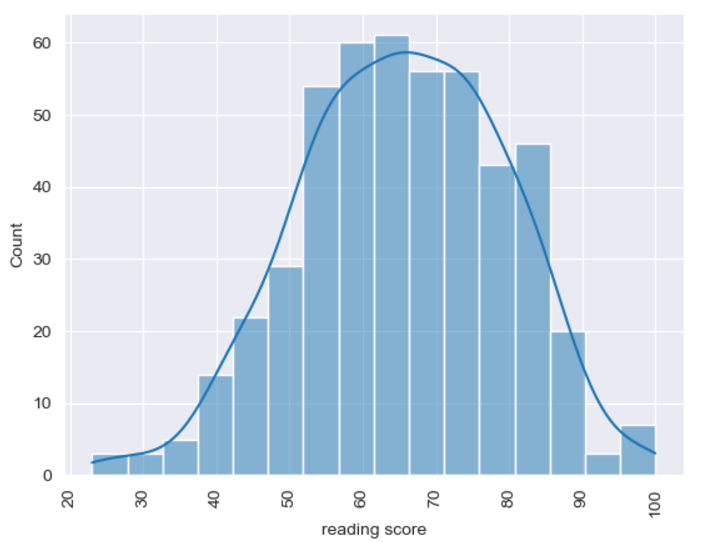
\includegraphics[width=\linewidth]{MaleStudentReadingScoreCurve.png}
        \caption{Male Students Reading Scores}
        \label{fig:MaleRead}
    \end{subfigure}
    \label{fig:FemaleMaleGraphsR}
\end{figure}
Coming back to the concerns regarding student Socioeconomic Status and its impact on student performance, we investigated how much the lunch program influenced the students' test scores.  Again, this is being used as another proxy for knowing a student's specific background, as only students whose families earn below a specified income level are eligible for the reduced/free lunch program.

Isolating the student performance by lunch program yielded the most significant results regarding impact of family SES and student performance. In Figure \ref{fig:lunch1} we have only included the Average Score chart because the differential was fairly consistent across all testing subjects. Average score was computed as a numerical average of the three individual subject scores.

\begin{figure}[H]
    \centering
    \caption{Student Average Scores Separated by Lunch Program}
    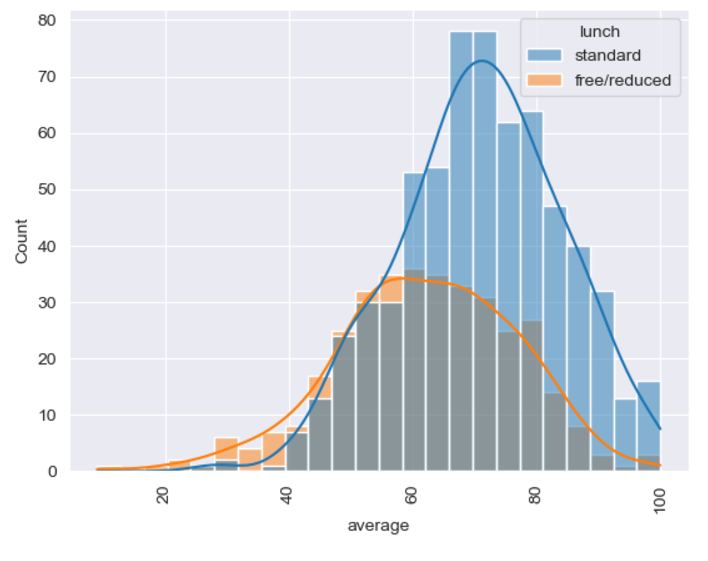
\includegraphics[width=0.75\linewidth]{StudentAvgScoresVSReducedLunch.png}
    \label{fig:lunch1}
\end{figure}
The students on the reduced/free lunch program had a mean score at least 10\% lower than those not on the plan as shown in Figure \ref{fig:lunch1}. Also of note is the percentage of students in this dataset which were on the reduced/free lunch program. There are 1000 students total in the dataset, with 645 not on the plan and 355 on the reduced/free lunch plan. Even though only 35\% of the dataset was on the reduced/free lunch plan, that is a significant proportion of a school population and would have a significant impact on needs of the overall population as discussed by the Office of Shared Accountability in Montgomery County Public Schools \cite{MCPSPoverty}.

Investigating how Race/Ethnicity played into student success, first we need to understand how many students were in each group.

\begin{table}[H]
    \centering
    \caption{Race/Ethnicity Student Representation Counts}
    \begin{tabular}{|c|c|}
    \hline
         Group Identifier & Student Count\\
         \hline\hline
         Group A & 89\\
         \hline
         Group B & 190\\
         \hline
         Group C & 319\\
         \hline
         Group D & 262\\
         \hline
         Group E & 140\\
         \hline
    \end{tabular}
    \label{tab:RaceCount}
\end{table}
Group C is the largest represented group while Group A is the smallest as seen in Table \ref{tab:RaceCount}. Within this limited context, we graphed the average scores of students grouped by their race/ethnicity identification. It is noteworthy in Figure \ref{fig:RaceScores} that the smallest represented group, the minority group by size, had the lowest mean of all the groups. It was also well below passing rate.  The two largest representative groups, Group C and Group D, have the highest mean scores, both hovering right around the passing rate. Group B performs similarly to Group A, with a low mean below passing rate, while Group E performs the best in the set with the highest mean of all the groups.
\begin{figure}[H]
    \centering
    \caption{Score Distribution Grouped By Race/Ethnicity}
    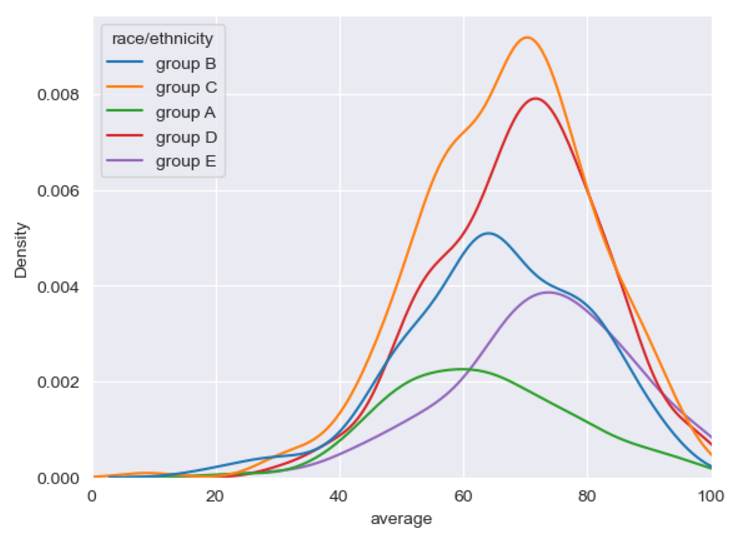
\includegraphics[width=0.5\linewidth]{RaceScoreDistribution.png}
    \label{fig:RaceScores}
\end{figure}
Lastly we looked at participation in a test preparation program and student success.  Completion of a test preparation program could also serve as a proxy for student socioeconomic status given most of these programs cost a significant amount of money, precluding lower socioeconomic status students from participating. However, not all mid and high SES families choose to utilize this as shown in the dataset participation rate.
Looking at the dataset split on participation in one of these test preparation courses, only a third of the dataset chose to complete a course. Those who did, however, saw improvements across all three test subjects.
\begin{figure}[H]
    \centering
    \caption{Participation in Test Prep Course Score Outcome}
    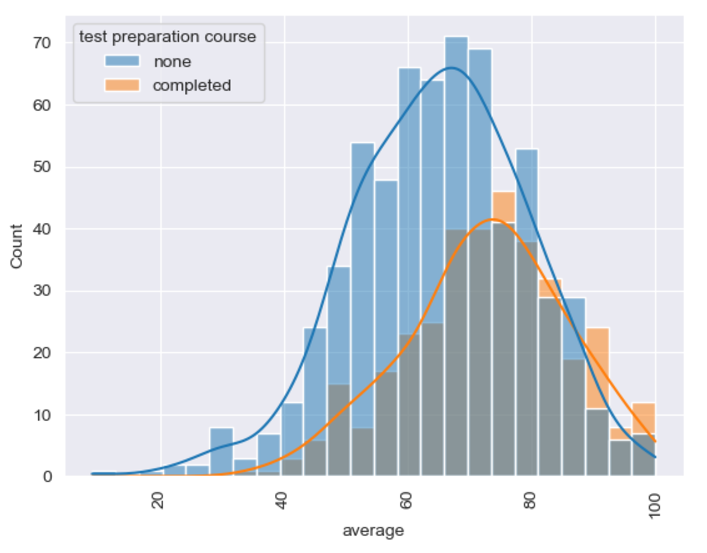
\includegraphics[width=0.7\linewidth]{TestPrepOverall.png}
    \label{fig:TestPrepOverall}
\end{figure}
Students who were able to complete a Test Preparation Program saw an overall average score 10 percentage points higher than their counterparts. More significantly, the difference between the two means placed them on opposite sides of the passing mark. Students who were able to complete one of these courses were significantly more likely to have passed all three assessments as seen in Figure \ref{fig:TestPrepOverall}.
\begin{figure}[H]
    \centering
    \caption{Test Preparation Course Participation vs Student Outcomes}
    \begin{subfigure}[b]{0.3\textwidth}
        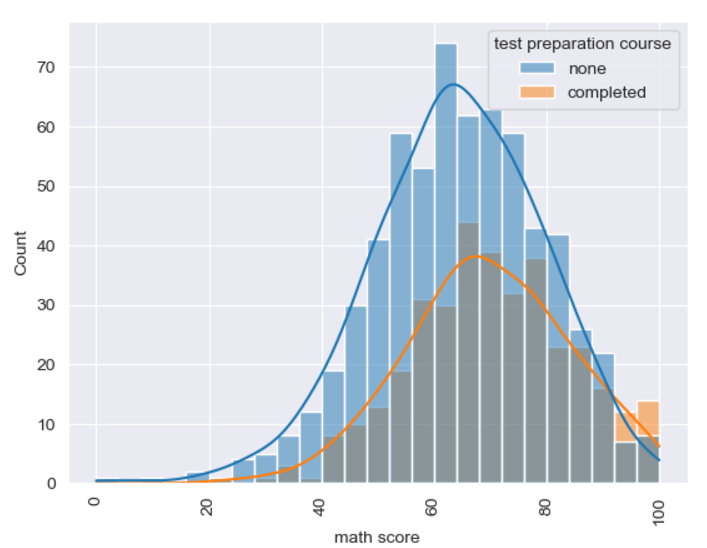
\includegraphics[width=\linewidth]{TestPrepMath.png}
        \caption{Test Prep vs. Math Scores}
        \label{fig:TestPrepMath}
    \end{subfigure}
    \begin{subfigure}[b]{0.3\textwidth}
        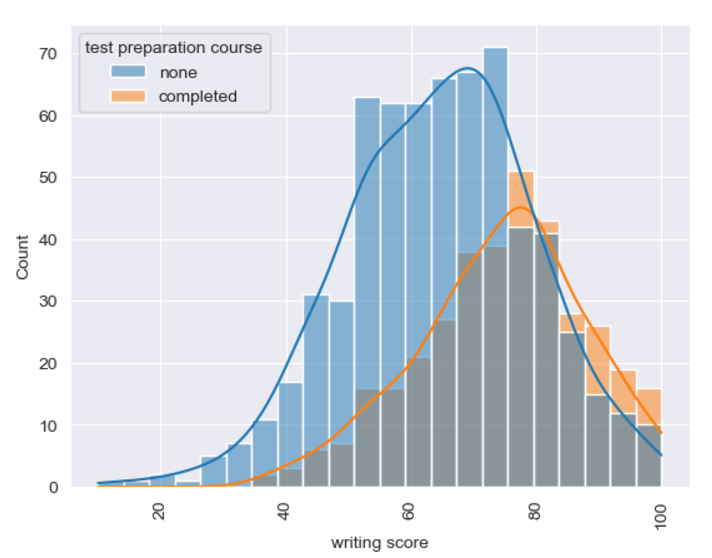
\includegraphics[width=\linewidth]{TestPrepWriting.png}
        \caption{Test Prep vs. Writing Scores}
        \label{fig:TestPrepWrite}
    \end{subfigure}
    \begin{subfigure}[b]{0.3\textwidth}
        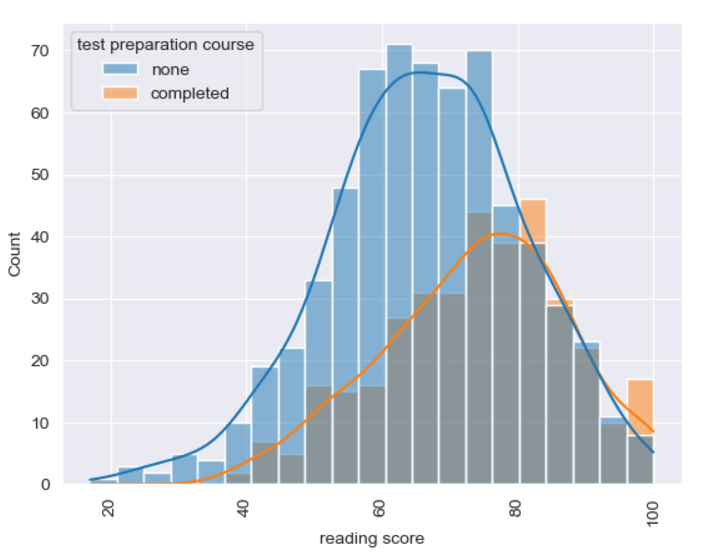
\includegraphics[width=\linewidth]{TestPrepReading.png}
        \caption{Test Prep vs. Reading Scores}
        \label{fig:TestPrepRead}
    \end{subfigure}
    \label{fig:TestPrepGraphs}
\end{figure}
When looking at specific subjects, Math scores showed the least improvement from a test preparation course, while Reading and Writing scores showed rather significant improvements as shown in Figure \ref{fig:TestPrepGraphs}.  Once again this is an indicator that family socioeconomic status plays a significant role in student outcomes. A family which is able to afford these programs provides yet another resource for their students to succeed while those whose families cannot afford it may be retained in grade or potentially passed forward with fewer of the skills to be successful in future academic endeavors.

\subsection{Data Preparation}
The chosen dataset \cite{dataset} is a generated dataset. It is not real student information, but created to replicate a student database. Therefore it cannot be used to infer anything about a specific population, but is available to demonstrate data analysis and machine learning model behaviors the techniques of which are transferable to real student information. This dataset consists of 8 columns, representing different elements of student data.  The second column of the Table \ref{tab:datasetCol} denotes valid values for that category.
\begin{table}[H]
    \centering
    \caption{Columns from Student Performance in Exams Dataset}
    \begin{tabular}{|l|p{8cm}|}
    \hline
        Gender & female/male\\
        \hline
        Race/Ethnicity & Group (A/B/C/D/E)\\
        \hline
        Parental Level of Education & Some High School, High School, Some College, Associate's Degree, Bachelor's Degree, Master's Degree\\
        \hline
        Lunch Program & Reduced/Free or None\\
        \hline
        Test Preparation Course & None/Completed\\
        \hline
        Math Assessment Score & Numeric from 0 to 100\\
        \hline
        Reading Assessment Score & Numeric from 0 to 100\\
        \hline
        Writing Assessment Score & Numeric from 0 to 100\\
        \hline
    \end{tabular}
    \label{tab:datasetCol}
\end{table}

The dataset is fairly evenly split between male and female students, skewing slightly more female at 52\% of the inputs. Students on the reduced/free lunch program make up about 1/3 of the dataset inputs, while those who completed a test preparation course also make up 1/3 of the dataset entries. Race/ethnicity groups are identified only by anonymous group letters, not by any specific identity. Group C is the largest representative group with 319 students, with Group A being the smallest with 89 students. Investigating the cross population of these racial groups with the available socioeconomic status could provide significant insights into which students require the most assistance to be successful, potentially revealing other systemic issues holding these students back.
The original dataset was checked for any null or duplicate entries and none were found. It was then evaluated for the values available per column. There were found to be three numerical columns, three more which had only binary values, and two which had multiple categorical entry options. These columns, minus the three score columns, were encoded for our model training step.
The training/test data set was then created from the encoded inputs. Different test sets were created to test each subject area independently. Test sets were split into train and evaluation in an 80/20 differential as is standard in test sets utilizing the Pareto Principle \cite{ParetoSplit}.
We elected to test the following models: Linear Regression, Lasso, Ridge, K Neighbors Regressor, Decision Tree, and Random Forrest Regressor. These models were among the most often sited in student outcome prediction data mining papers as discussed in \cite{MLMoodle} and \cite{dataMineLit}. Utilizing the same prepared input data, we ran a training loop where each model was trained and then evaluated. The models were evaluated utilizing Root Mean Squared Error, Mean Absolute Error, and R2 score as is appropriate for a regression task and discussed in \cite{measuremetrics}.
Each standardized test score column was individually removed as the prediction target, creating three unique test set pairs. The models were then trained on the appropriate training set, and evaluated on the test set split. There was some parameter fine tuning performed on the models to increase R2 score.  Originally we also included Logistical Regression in the model list, but upon testing found it was not converging. We performed a GridSearchCV as well and found a consistent issue with convergence. Therefore, this model was removed from our testing analysis.
Further testing was then done removing different columns from the input data to test how much each influenced each model's prediction behavior. Relative to the hypothesis that socioeconomic status was a major influencer in a student's success, we decided to remove individual columns indicated as possible proxies for SES, and which were found to have some influence during our data analysis stage. Each of the following was removed from various iterations of the training and test set individually to evaluate how much influence they had on the models: Parental Level of Education, Race/Ethnicity, Lunch, Gender, and Test Preparation Course. We also ran one test with all the standardized scores removed.
\section{Results and Analysis}
Original intentions were to test four linear models and three non-linear models. After attempting numerous parameter settings to encourage the Logistical Regression model to converge with the provided data, it was removed from analysis. The results from this model are included in Table \ref{tab:InitModelPerfMath} to illustrate the low test results prior to removal. We ran GridSearchCV in an attempt to increase the model's likelihood of convergence, but were not successful.
Performance of the models was measured with MAE, RMSE, and R2 score. Since the output is continuous, these were the best metrics for measure model fit for the task.
Initial testing ran all models through training and evaluation for each subject score individually. There were differences between the models on which subject was a best fit.  It was also noted that the unconstrained DecisionTree had a decided overfit problem. It would achieve 100\% R2 score on the training data, but exhibit a 20\% drop on the evaluation data as seen Table \ref{tab:InitModelPerfMath}.

\begin{table}[H]
    \centering
    \caption{Model Performance Predicting Math Scores}
    \begin{tabular}{|c|c|c|c|}
    \hline
         Model & RMSE & MAE & R2 Score\\
         \hline\hline
         Linear Regression & 5.3940 & 4.2207 & 0.8804\\
         \hline
         Lasso & 6.5197 & 5.1579 & 0.8253\\
         \hline
         Ridge & 5.3905 & 4.2180 & 0.8806\\
         \hline
         K-Neighbors Regressor & 7.5083 & 5.8380 & 0.7683\\
         \hline
         Decision Tree & 7.9057 & 6.5200 & 0.7143\\
         \hline
         RandomForestRegressor & 5.9211 & 4.6468 & 0.8559\\
         \hline
         Logistical Regression & 9.8430 & 7.5950 & 0.6019\\
         \hline
    \end{tabular}
    \label{tab:InitModelPerfMath}
\end{table}
Both Linear Regression and Ridge models performed best of this group on predicting the Math Score being able to explain 88\% of the variance in the scores. Both models were also least likely of the group to be influenced by outliers, as demonstrated by their RSME values, and both had less than 5 points variation from the actual score value per their MAE value.  This is an acceptable score deviation for predicting which students will benefit from more intervention.
In this iteration we did not constrain the Decision Tree model. Training results indicated significant overfitting, however. Upon retraining and evaluating the model with min\_samples\_leaf set to 8, Decision Tree improved significantly. The max\_depth parameter was also tested with various values, in combination with and without min\_samples\_leaf, but proved not to have as much influence as min\_samples\_leaf as seen in Table \ref{tab:DecTreeControlled}.

\begin{table}[H]
    \centering
    \caption{Decision Tree after parameter adjustment}
    \begin{tabular}{|c|c|c|c|}
    \hline
        Model & RMSE & MAE & R2 Score\\
        Decision Tree min\_sample\_leaf=8 & 6.5365 & 5.2004 & 0.8244\\
        \hline
    \end{tabular}
    \label{tab:DecTreeControlled}
\end{table}
Holding these settings consistent for the same models, but predicting the Writing score, yielded the same results as to top performing models. The overall performance was actually better. See Table \ref{tab:InitModelPerfWrite}
\begin{table}[H]
    \centering
    \caption{Model Performance Predicting Writing Scores}
    \begin{tabular}{|c|c|c|c|}
    \hline
         Model & RMSE & MAE & R2 Score\\
         \hline\hline
         Linear Regression & 3.8715 & 3.2117 & 0.9378\\
         \hline
         Lasso & 4.9256 & 3.8964 & 0.8993\\
         \hline
         Ridge & 3.8711 & 3.2113 & 0.9378\\
         \hline
         K-Neighbors Regressor & 5.3888 & 4.2190 & 0.8795\\
         \hline
         Decision Tree & 5.1687 & 4.0136 & 0.8892\\
         \hline
         RandomForestRegressor & 4.4709 & 3.6056 & 0.9171\\
         \hline
    \end{tabular}
    \label{tab:InitModelPerfWrite}
\end{table}
\begin{table}[H]
    \centering
    \caption{Model Performance Predicting Reading Scores}
    \begin{tabular}{|c|c|c|c|}
    \hline
         Model & RMSE & MAE & R2 Score\\
         \hline\hline
         Linear Regression & 4.3275 & 3.4881 & 0.9172\\
         \hline
         Lasso & 4.6350 & 3.6941 & 0.9051\\
         \hline
         Ridge & 4.3213 & 3.4831 & 0.9175\\
         \hline
         K-Neighbors Regressor & 6.2467 & 4.6870 & 0.8276\\
         \hline
         Decision Tree & 4.9466 & 3.9183 & 0.8919\\
         \hline
         RandomForestRegressor & 4.8310 & 3.6323 & 0.9093\\
         \hline
    \end{tabular}
    \label{tab:InitModelPerfRead}
\end{table}
Similar outputs were found when testing for Reading Score prediction as shown in Table \ref{tab:InitModelPerfRead} although the models were able to perform best with the Writing data than for either of the other two standardized test sets.
We wanted to perform evaluation runs which included removing more of the columns deemed indicative of a student's socioeconomic status. These were also all columns which seemed to have a correlation to a student's success in the Data Analysis stage of our testing.
The first additional column we removed was the Lunch column. Included below in Table \ref{tab:ReadNoLunch} are the results from the Reading Score prediction with this additional column removed.
\begin{table}[H]
    \centering
    \caption{Model Performance on Reading Score Prediction with Lunch Column Removed}
    \begin{tabular}{|c|c|c|c|}
    \hline
         Model & RMSE & MAE & R2 Score\\
         \hline\hline
         Linear Regression & 4.3202 & 3.4668 & 0.9175 \\
         \hline
         Lasso & 4.6350 & 3.6941 & 0.9051 \\
         \hline
         Ridge & 4.3131 & 3.4606 & 0.9178 \\
         \hline
         K-Neighbors Regressor & 6.0851 & 4.6410 & 0.8364 \\
         \hline
         Decision Tree & 4.8587 & 3.84848 & 0.8957 \\
         \hline
         RandomForestRegressor & 4.5058 & 3.5853 & 0.9103 \\
         \hline
    \end{tabular}
    \label{tab:ReadNoLunch}
\end{table}
Interestingly, comparing Table \ref{tab:ReadNoLunch} to Table \ref{tab:InitModelPerfRead} yields not much of a model performance degradation. While the data analysis indicates this metric is a big determiner, the models are not indicating it is an important metric for training and prediction.
Removing Race/Ethnicity or gender yield a similar result to Lunch. Removing Parental Level of Education yielded a slight degradation of less than 1\% in R2 score fairly uniformly across all models.  However, upon deciding to test removing all other standardized test scores and predicting the Math score, the models could not achieve an R2 score above 10\%.  Clearly, the most important metric of all is prior performance, as was indicated by \cite{7008697}. As found by Slim et al., models provided with even a single semester of prior performance are able to predict student success fairly accurately, becoming more accurate as more information is available. Therefore it was not surprising that removing all prior performance data caused the models to be unable to predict with any success.

\section{Conclusion}
We set out to demonstrate there are Machine Learning models capable of being added to the arsenal of tools a school can utilize to identify students who would benefit from additional intervention. We also intended to identify which metrics might be of more influence to both student success and model training.
Data Analysis indicated information such as the student's participation in a reduced/free lunch program, or the educational attainment of the student's parents would be important factors.  However, once we implemented the model testing we found this not to be as important. The most important information we could have about a student for the models to predict successfully was prior academic performance data.
There will always be a strong correlation between a student's prior performance and their future performance. Relying on prior academic record alone would yield a higher number of students needing intervention than most schools have resources to provide. In light of having resource limitations, we propose a combination of the data analysis points and model predictions. There is expansion opportunity in this field of study, including learning how certain background and societal metrics relate to one another. Of interest is how some of the socioeconomic indicators interplay with elements such as parental educational attainment, stable households, access to quality pre-K and reading materials, and student success. 
With much opportunity to explore Data Mining and Student Attainment, hopefully more students will be identified and utilize the limited resources a school has to help them succeed. 

\bibliographystyle{apacite} % APA citation style
\bibliography{bibliography}  % Reference to your .bib file

\end{document}